\documentclass[twoside,twocolumn]{article}
\usepackage{amsmath}
\usepackage{amssymb}
\usepackage[hmarginratio=1:1,top=32mm,columnsep=20pt]{geometry}
\usepackage[hang, small,labelfont=bf,up,textfont=it,up]{caption} 
\usepackage{booktabs}
\usepackage{enumitem}
\setlist[itemize]{noitemsep}
\usepackage{abstract}
\renewcommand{\abstractnamefont}{\normalfont\bfseries}
\renewcommand{\abstracttextfont}{\normalfont\small\itshape}
\usepackage{titlesec}
\renewcommand\thesection{\Roman{section}}
\renewcommand\thesubsection{\Alph{subsection}}
\renewcommand\thesubsubsection{\arabic{subsubsection}}
\titleformat{\section}[block]{\normalsize\bfseries\scshape\centering}{\thesection.}{1em}{}
\titleformat{\subsection}[block]{\normalsize\bfseries\centering}{\thesubsection.}{1em}{}
\titleformat{\subsubsection}[block]{\normalsize\centering}{\thesubsubsection.}{1em}{}
\usepackage{fancyhdr}
\pagestyle{fancy}
\fancyhead{}
\fancyhead[C]{Computational Physics Homework $\bullet$ May 2018 $\bullet$ Vol. I, No. 4}
\usepackage{titling}
\usepackage{hyperref}
\hypersetup{unicode}
\AtBeginShipoutFirst{\input{zhwinfonts.tex}}
\usepackage{bm}
\usepackage{braket}
\usepackage{CJKutf8}
\usepackage{xcolor}
\usepackage{dcolumn}
\usepackage{graphicx}
\usepackage{indentfirst}
\usepackage{listings}
\usepackage[toc, page, title, titletoc, header]{appendix}
\definecolor{grey}{rgb}{0.8,0.8,0.8}
\definecolor{darkgreen}{rgb}{0,0.3,0}
\definecolor{darkblue}{rgb}{0,0,0.3}
\def\lstbasicfont{\fontfamily{pcr}\selectfont\footnotesize}
\lstset{
	numbers=left,
	numberstyle=\small,
	showstringspaces=false,
	showspaces=false,
	tabsize=4,
	frame=single,
	basicstyle={\footnotesize\lstbasicfont},
	keywordstyle=\color{darkblue}\bfseries,
	identifierstyle=,
	commentstyle=\color{darkgreen},
	stringstyle=\color{black}
}
\lstloadlanguages{C,C++,Fortran,Java,Matlab,Mathematica,Python}
\setlength{\parindent}{2em}
\begin{document}
\begin{CJK*}{UTF8}{gkai}
%----------------------------------------------------------------------------------------
%	TITLE SECTION
%----------------------------------------------------------------------------------------

\setlength{\droptitle}{-4\baselineskip} % Move the title up
\pretitle{\begin{center}\Huge\bfseries} % Article title formatting
	\posttitle{\end{center}} % Article title closing formatting
\title{计算物理第四次作业} % Article title
\author{
	\textsc{梁旭民}\thanks{\noindent 指导老师:齐新老师} \\[1ex] % Your name
	\normalsize Cuiying Hornors College, Lanzhou University \\ % Your institution
	\normalsize \href{mailto:liangxm15@lzu.edu.cn}{liangxm15@lzu.edu.cn} % Your email address
}
\date{}
\renewcommand{\maketitlehookd}{
	\begin{abstract}
		本次计算物理作业有两个问题:第一个问题是学习Sherman-Morrison公式及Sherman-Morrison-Woodbury公式,并利用公式将对于循环三对角线性方程组的求解问题转化为对于三对角线性方程组的求解,从而使得问题得到简化。第二个问题则是利用有限差分的方法求解一个具体的物理问题:第一类边界条件下的Poisson-Boltzman方程从而求解出等离子体孤波的电势分布情况。
	\end{abstract}
}
\maketitle

%----------------------------------------------------------------------------------------
%	SECTION 1
%----------------------------------------------------------------------------------------

\section{Sherman-Morrison公式}
\subsection{问题描述}
利用Sherman-Morrison公式作为Gauss消元法的修正,求解循环三对角矩阵的逆,从而求解循环三对角线性方程组$Ax=r$并且在以上基础上了解woodbury公式
\subsection{问题分析}
\subsubsection{Sherman-Morrison公式表述}
设$A\in \mathbb{R}^{n\times n}$是一个可逆方阵并且$u,v\in \mathbb{R}^{n}$是列向量。当且仅当$I+v^{T}A^{-1}u\neq 0$ ,则有$A+uv^{T}$是可逆的,且它的逆可以写成
\begin{equation*}
	(A+uv^{T})^{-1}=A^{-1}-\frac{A^{-1}uv^{T}A^{-1}}{I+v^{T}A^{-1}u}
\end{equation*}
其中,$uv^{T}$是两个向量$u,v$的外积。
\subsubsection{Sherman-Morrison公式证明}
证明必要性。当且仅当$XY=YX=I$,矩阵Y(Sherman-Morrison公式的右边)是矩阵X($A+uv^{T}$)的逆矩阵。

我们先验证矩阵Y满足$XY=I$,则有
\begin{equation*}
	\begin{aligned}
		XY
		&=(A+uv^{T})\left(A^{-1}-\frac{A^{-1}uv^{T}A^{-1}}{ 1+v^{T}A^{-1}u}\right)\\
		&=AA^{-1}+uv^{T}A^{-1}\\&-\frac{AA^{-1}uv^{T}A^{-1}+uv^{T}A^{-1}uv^{T}A^{-1}}{ 1+v^{T}A^{-1}u}\\
		&=I+uv^{T}A^{-1}\\&-\frac{uv^{T}A^{-1}+uv^{T}A^{-1}uv^{T}A^{-1}}{ 1+v^{T}A^{-1}u}\\
		&=I+uv^{T}A^{-1}\\&-\frac{u(1+v^{T}A^{-1}u)v^{T}A^{-1}}{ 1+v^{T}A^{-1}u}\\
		&=I+uv^{T}A^{-1}-uv^{T}A^{-1}\\
		&=I
	\end{aligned}
\end{equation*}
类似的,可以验证
\begin{equation*} YX=\left(A^{-1}-\frac{A^{-1}uv^{T}A^{-1}}{ 1+v^{T}A^{-1}u}\right)(A+uv^{T})=I. 
\end{equation*}

证明充分性。假设$u\neq 0$,则有
\begin{equation*}
	(A+uv^{T})A^{-1}u=u+uv^{T}A^{-1}u=(I+v^{T}A^{-1}u)u
\end{equation*}

因此,假设$A+uv^{T}$是可逆矩阵,则$(A+uv^{T})A^{-1}$作为可逆矩阵的乘积,也是可逆矩阵。因此,通过假设$u\neq 0$,我们可以得到$(A+uv^{T})A^{-1}u\neq 0$。
\subsubsection{Woodbury公式表述}
设$A\in \mathbb{R}^{n\times n}$是一个可逆方阵并且$u,v\in \mathbb{R}^{n}$是列向量。当且仅当$I+v^{T}A^{-1}u\neq 0$ ,则有$A+uv^{T}$是可逆的。如果$A+uv^{T}$是可逆的,且它的逆可以写成
\begin{equation*}
	(A+uv^{T})^{-1}=A^{-1}-A^{-1}u(I+v^{T}A^{-1}u)v^{T}A^{-1}
\end{equation*}
\subsubsection{Sherman-Morrison-Woodbury公式证明}
设$(A+uv^{T})x=r$,则有
\begin{equation*}
	A^{-1}(A+uv^{T})x=x+A^{-1}uv^{T}x=A^{-1}r
\end{equation*}
若假设
\begin{equation*}
	\left\{
	\begin{aligned}
		&A^{-1}x=z\\
		&A^{-1}r=y
	\end{aligned}
	\right.
\end{equation*}
则可以得到
\begin{equation*}
	x+zv^{T}x=y
\end{equation*}
左右两边同时左乘$v^{T}$,并令$\alpha=v^{T}x$,则有
\begin{equation*}
	\alpha+v^{T}z\alpha=v^{T}y
\end{equation*}
可以解得
\begin{equation*}
	\alpha=\frac{v^{T}y}{I+v^{T}z}
\end{equation*}
代入$x+\alpha z=y$,则有
\begin{equation*}
	\begin{aligned}
		x&=y-\alpha z\\
		&=A^{-1}r-A^{-1}u(I+v^{T}A^{-1}u)^{-1}v^{T}y\\
		&=A^{-1}r-A^{-1}u(I+v^{T}A^{-1}u)^{-1}v^{T}A^{-1}r\\
		&=[A^{-1}-A^{-1}u(I+v^{T}A^{-1}u)^{-1}v^{T}A^{-1}]r
	\end{aligned}
\end{equation*}
因此证明
\begin{equation*}
	(A+uv^{T})=A^{-1}-A^{-1}u(I+v^{T}A^{-1}u)^{-1}v^{T}A^{-1}
\end{equation*}
\subsubsection{利用Sherman-Morrison公式求解循环三对角线性方程组}
求解的循环三对角线性方程组为
\begin{equation*}
	Ax=r
\end{equation*}
其中$A\in \mathbb{R}^{n\times n}$为可逆矩阵,其具体形式如下
\begin{equation*}
	A=
	\begin{bmatrix} 
		b_1&c_1&0&\cdots&0&a_1\\
		a_2&b_2&c_2&0&\vdots&0\\
		0&\ddots&\ddots&\ddots&0&\vdots\\
		\vdots&\vdots&a_{n-2}&b_{n-2}&c_{n-2}&0\\
		0&\cdots&\cdots&a_{n-1}&b_{n-1}&c_{n-1}\\
		c_n&0&\cdots&0&a_n&b_n
	\end{bmatrix}
\end{equation*}
而矢量$r=(r_{1},r_{2},\cdots,r_{n})^{T}$为已知,其中$x=(x_{1},x_{2},\cdots,x_{n})^{T}$为待求未知数。

若构造三对角矩阵B为
\begin{equation*}
	\begin{bmatrix} 
		b_1-\gamma&c_1&0&\cdots&0&0\\
		a_2&b_2&c_2&0&\vdots&0\\
		0&\ddots&\ddots&\ddots&0&\vdots\\
		\vdots&\vdots&a_{n-2}&b_{n-2}&c_{n-2}&0\\
		0&\cdots&\cdots&a_{n-1}&b_{n-1}&c_{n-1}\\
		0&0&\cdots&0&a_n&b_n-\frac{a_1c_n}{\gamma}\end{bmatrix}
\end{equation*}
使其满足$A=B+uv^{T}$,且有$1+v^{T}B^{-1}u\neq 0$。\\
其中$u,v\in \mathbb{R}^{n}$为列向量,可以写成
\begin{equation*}
	\left\{
	\begin{aligned}
		&u=(\gamma,0,0,\cdots,c_{n})^{T}\\
		&v=(1,0,0,\cdots,\frac{a_{1}}{\gamma})^{T}
	\end{aligned}
	\right.
\end{equation*}
则原线性方程组变成
\begin{equation*}
	(B+uv^{T})x=r
\end{equation*}
可以将该线性方程组分解成以下两个三对角线性方程组,通过求解以下两个三对角线性方程组
\begin{equation*}
	\left\{
	\begin{aligned}
		&By=r\\
		&Bz=u
	\end{aligned}
	\right.
\end{equation*}
利用Sherman-Morrison公式,便可以得到原线性方程组的解为
\begin{equation*}
	x=y-\frac{v^{T}y}{1+v^{T}z}z
\end{equation*}
\subsubsection{验证原方程解}
将$x=y-\frac{v^{T}y}{1+v^{T}z}z$代入原线性方程组,则有
\begin{equation*}
	\begin{aligned}
		&(B+uv^{T})x\\
		&=(B+uv^{T})(y-\frac{v^{T}y}{1+v^{T}z}z)\\
		&=By+uv^{T}y-\frac{v^{T}y}{1+v^{T}z}Bz-\frac{v^{T}y}{1+v^{T}z}uv^{T}z\\
		&=r+uv^{T}y-\frac{v^{T}yu+v^{T}yuv^{T}z}{1+v^{T}z}\\
		&=r+uv^{T}y-\frac{(1+v^{T}z)v^{T}yu}{1+v^{T}z}\\
		&=r+uv^{T}y-uv^{T}y\\
		&=r
	\end{aligned}
\end{equation*}

%----------------------------------------------------------------------------------------
%	SECTION 2
%----------------------------------------------------------------------------------------

\section{一维Poisson-Bolzman方程}
\subsection{问题描述}
求解第一类边界条件下(边界$\phi=0$)的一维Poisson-Boltzman方程,计算等离子体孤波的电势。
\begin{equation*}
	\frac{\partial^{2}\phi}{\partial x^{2}}=\mu \mathrm{e}^{\phi}-Zn_{i}
\end{equation*}
其中,$\mu=1$,$Z=1$,离子密度$n_{i}(x)$为
\begin{equation*}
	n_{i}(x)=1+3\varepsilon^{2}u_{0} \mathrm{sech}^{2}\frac{\varepsilon\sqrt{\mu_{0}}[x-x_{0}]}{2}
\end{equation*}

其形状大致见FIG. 1.(纵坐标为电势$\phi$,但在$\varepsilon^{2}\ll 1$时,$\phi=n_{i}-1$)

\begin{figure}[h]
	\centering
	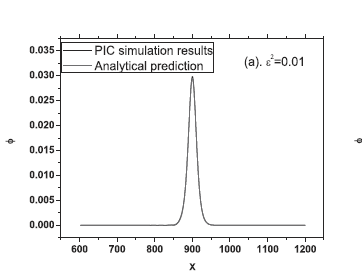
\includegraphics[width=0.7\linewidth]{./figure/figure1.png}
	\caption{离子浓度分布}
	\label{fig:figure1}
\end{figure}
其中,$u_{0}=1$。
\subsection{问题分析}
\subsubsection{简介}
Poisson- Boltzmann方程是用来计算电解质溶液中离子浓度和电荷密度分布的一个微分方程。其基本形式为(单位为高斯单位制)
\begin{equation*}
\displaystyle \nabla ^{2}\phi ({\textbf {r}})=-{\frac {4\pi }{\epsilon }}\sum _{i}c_{i}^{0}z_{i}qe^{-\beta z_{i}q\phi ({\textbf {r}})}
\end{equation*}
其中,$\phi$是体系的电势,$\epsilon$是溶液的介电常数,$c_{i}^{0}$和$z_{i}$分别为第i种离子的体相浓度和电荷,$\beta =\frac{1}{k_{B}T}$, 其中$k_{B}$是Boltzman常数。该方程的雏形最早出现于双电层理论的Gouy-Chapman模型中,在这个模型中离子在电极表面附近的分布被认为是遵从玻尔兹曼分布。

如今该方程被广泛运用于各种电解质溶液体系性质的计算和分子模拟中,特别是生物体系中各种大分子(例如核酸和蛋白质)在溶液中电荷分布和溶解自由能的计算。
\subsubsection{原理}
Poisson-Boltzman方程实际上是通过对体系的平均力势能(Potential of Mean Force, PMF)作平均场近似而得到。从电解质溶液体系的Poisson方程出发
\begin{equation*}
\nabla ^{2}\phi ({\textbf {r}})=-{\frac {4\pi }{\epsilon }}\sum _{i}z_{i}qc_{i}({\textbf {r}})
\end{equation*}
而第i种离子的浓度函数$c_{i}({\textbf {r}})$可以写成
\begin{equation*}
c_{i}({\textbf {r}})=c_{i}^{0}e^{{-\beta w_{i}({\textbf {r}})}}
\end{equation*}
其中$w_{i}({\textbf {r}})$即为第i种离子的平均力势能。

在平均场近似中,忽略离子间的关联,令平均力势能近似等于该离子的电势能
\begin{equation*}
w_{i}({\textbf {r}})\simeq z_{i}q\phi ({\textbf {r}}),
\end{equation*}
即得到Poisson-Boltzman方程。
\subsubsection{求解}
Poisson-Boltzman方程是一个非线性偏微分方程,除了在特定简化体系(如Gouy-Chapman模型)中能求得解析解外,一般采用数值解法,例如有限差分法或者有限元方法。

当离子的电势能绝对值较小时,即$ \beta z_{i}q\phi ({\textbf {r}})<<1$时,可以把泊松-玻尔兹曼方程中的指数项仅展开到一阶
\begin{equation*}
\mathrm{e}^{{-\beta z_{i}q\phi ({\textbf {r}})}}\simeq 1-\beta z_{i}q\phi ({\textbf {r}})
\end{equation*}
即可得到Debye-Hückel方程
\begin{equation*}
\nabla ^{2}\phi ({\textbf {r}})+\kappa ^{2}\phi ({\textbf {r}})=0
\end{equation*}
其中$\kappa ^{2}={\frac {4\pi z_{i}^{2}q^{2}c_{i}^{{0}}}{\epsilon k_{B}T}}$。Debye-Hückel方程是一个线性偏微分方程,易于求解。在稀溶液中,德拜-休克尔方程对于泊松-玻尔兹曼方程而言是很好的近似。
\subsubsection{应用与局限}
Poisson-Boltzman方程的优势在于将溶液中的水简化为具有均一介电常数的电介质,这种隐式溶剂(Implicit Solvent)的处理方法极大地简化了生物大分子溶液体系中的模拟和计算。例如,在生物大分子溶液的分子动力学模拟中,体系可以只包含生物大分子,而忽略水分子和其他离子,并采用Poisson-Boltzman方程来获得大分子的受力。类似地,对于溶解自由能的计算,来自溶剂的贡献可以使用广义Born模型来处理,而离子的贡献则可以采用Poisson-Boltzman方程 。

Poisson-Boltzman方程的缺点在于其所使用的平均场近似,当溶液中出现一定浓度高价离子导致离子间相互作用和关联增强,Poisson-Boltzman方程的解将无法解释一些 由关联所产生的现象,比如带相同电荷的物体在高价盐溶液中相互吸引,以及带电胶体在高价盐溶液中的电泳呈现电荷反转,这些现象必须考虑离子间的关联才能得到合理解释。
\subsection{算法设计}
选取$N=30000$,$dx=0.01$,使得求解范围为$0-300$:

1.\quad  首先利用二阶微商差分公式
\begin{equation*}
\frac{\mathrm{d}^{2}\phi}{\mathrm{d}x^{2}}= \frac{\phi_{i-1}-2\phi_{i}+\phi_{i+1}}{\mathrm{d}x^{2}}
\end{equation*}
将Poisson-Boltzman方程左端化为一个 $N\times N$ 的三对角行列式。再将密度$n_{i}$离散化,得到右端$\rho (1:30000)$数组。

2.\quad 将Poisson-Boltzman方程右端指数项做一阶泰勒展开 
\begin{equation*}
\mathrm{e}^{\phi}=1+\phi
\end{equation*}
并将其代入Poisson-Boltzman方程,利用三对角矩阵求解,得到一阶线性近似的电势
\begin{equation*}
\phi_{n}^{(1)}\quad n=1,2,...,30000
\end{equation*}

3.\quad 得到$\phi_{n}^{(1)}$后,利用
\begin{equation*}
\begin{aligned}
\mathrm{e}^{\phi^{(2)}}
&=\mathrm{e}^{\phi^{(1)}+(\phi^{(2)}-\phi^{(1)})}\\
&=\mathrm{e}^{\phi^{(1)}}\mathrm{e}^{(\phi^{(2)}-\phi^{(1)})}\\
&=\mathrm{e}^{\phi^{(1)}}[1+(\phi^{(2)}-\phi^{(1)})]
\end{aligned}
\end{equation*}
再次将Poisson-Boltzman方程右端线性化,再解新的对三角矩阵得到$\phi_{n}^{(2)}$,如此往复
\begin{equation*}
\mathrm{e}^{\phi^{(n+1)}}=\mathrm{e}^{\phi^{(n)}}[1+(\phi^{(n+1)}-\phi^{(n)})]
\end{equation*}
数次迭代后即可线性逼近非线性Poisson-Boltzman方程解。

4.\quad 初步校验程序正确性。$\varepsilon^{2}$为小量,分别取值$0.01,0.1,0.3$,在极小时候$\phi=n_{i}-1$,电势和密度形状完全相同,随着$\varepsilon^{2}$增大,电势密度开始出现差别。
\subsection{计算结果}
我们现将$\varepsilon^{2}=0.01,0.1,0.3$的数据存入excel中,然后使用Python的Matplotlib包将离子浓度分布图像及Poisson-Boltzman解的图像输出。
离子浓度分布随$\varepsilon^{2}$图像绘制见Figure 2.

\begin{figure}[h]
\centering
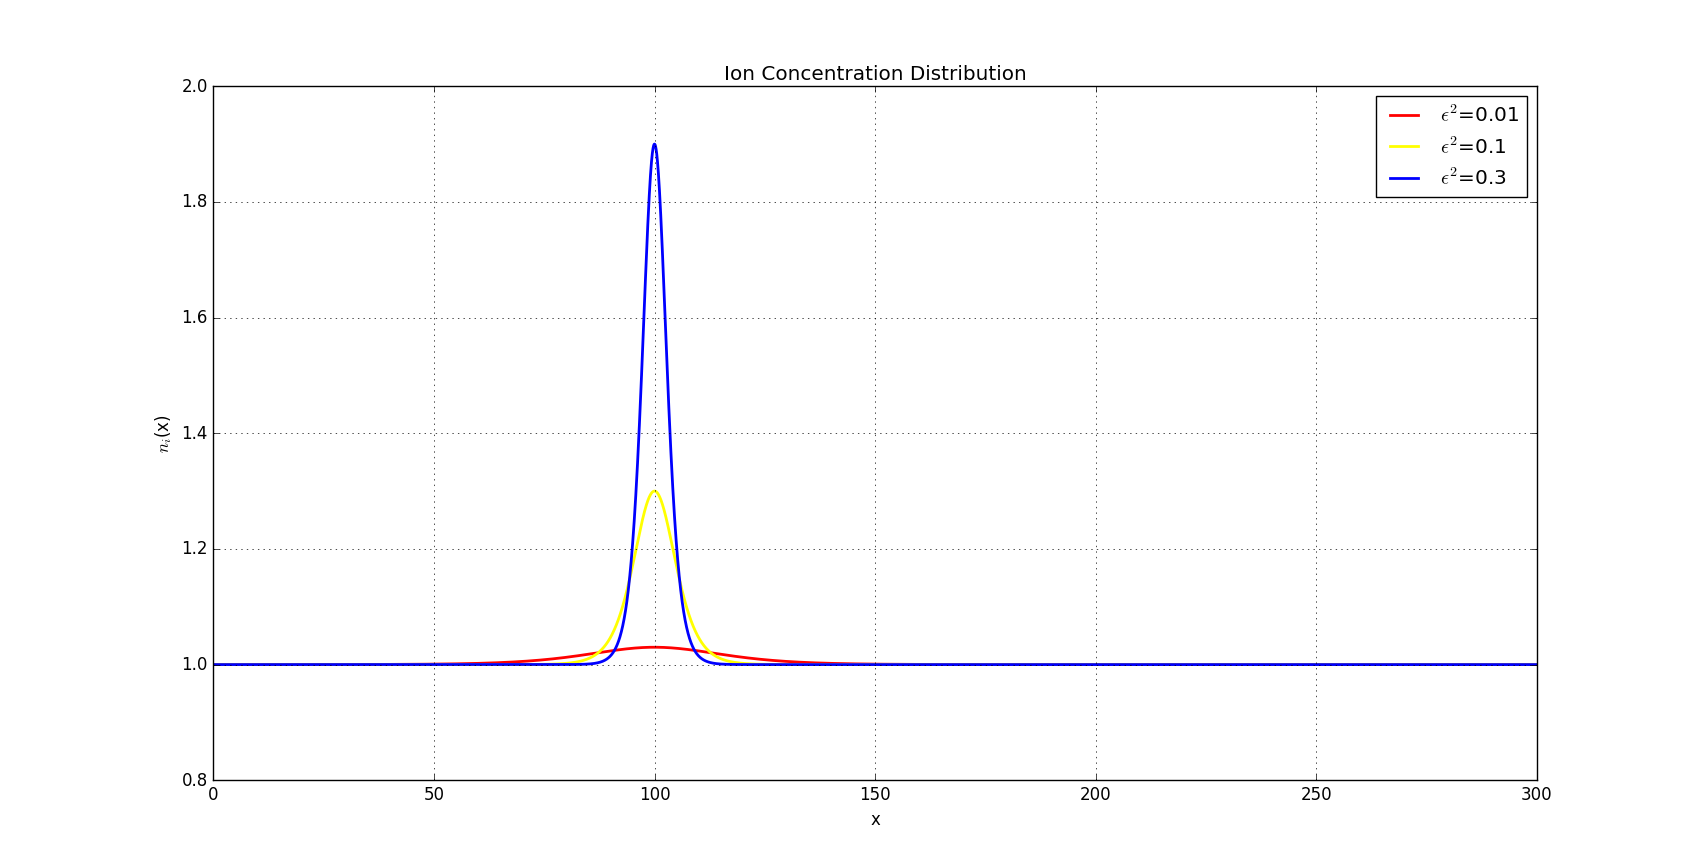
\includegraphics[width=1.0\linewidth]{figure/figure2}
\caption{离子浓度分布图}
\label{fig:figure2}
\end{figure}

Poisson-Boltzman方程求解结果见Figure 3.
\begin{figure}[h]
\centering
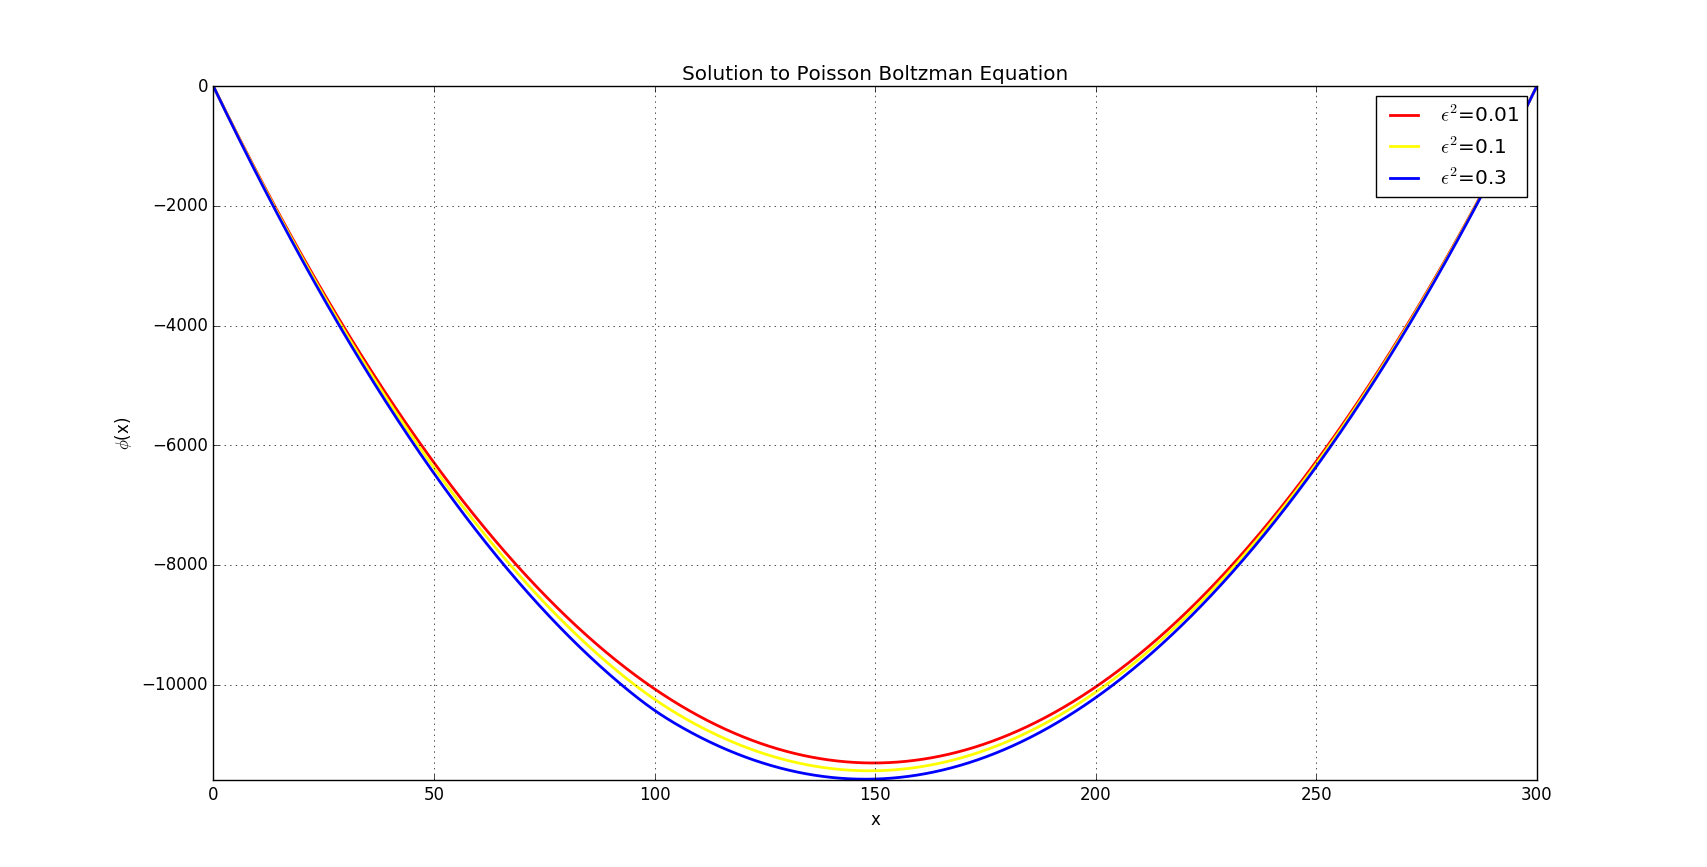
\includegraphics[width=1.0\linewidth]{figure/figure3}
\caption{Poisson-Boltzman方程解}
\label{fig:figure3}
\end{figure}
通过图像我们可以发现,随着$\varepsilon^{2}$的增大,Poisson-Boltzman方程的解趋势基本不变,但极小值越来越小。

%----------------------------------------------------------------------------------------
%	APPENDICES SECTION
%----------------------------------------------------------------------------------------

\newpage
\onecolumn
\begin{appendices}

\section{求解循环三对角矩阵的逆}
Here is the program to solve the linear equations.\\
\textbf{\textcolor[rgb]{0.98,0.00,0.00}{Input Python source:}}
\lstinputlisting[language=Python]{./program/Sherman_Morrison.py}
\newpage
\section{求解Poisson-Boltzman方程}
Here is the program to solve the Poisson-Boltzman equations.\\
\textbf{\textcolor[rgb]{0.98,0.00,0.00}{Input Python source:}}
\lstinputlisting[language=Python]{./program/Poisson_Boltzman.py}
\newpage
\section{离子浓度分布作图部分}
Here is the program to draw the figure.\\
\textbf{\textcolor[rgb]{0.98,0.00,0.00}{Input Python source:}}
\lstinputlisting[language=Python]{./program/draw1.py}
\newpage
\section{Poisson-Boltzman解作图部分}
Here is the program to draw the figure.\\
\textbf{\textcolor[rgb]{0.98,0.00,0.00}{Input Python source:}}
\lstinputlisting[language=Python]{./program/draw2.py}

\end{appendices}

%----------------------------------------------------------------------------------------
%	REFERENCE
%----------------------------------------------------------------------------------------

\newpage
\renewcommand\refname{参考文献}
\begin{thebibliography}{99}
\bibitem{ref1} Sherman, Jack; Morrison, Winifred J. (1949). "Adjustment of an Inverse Matrix Corresponding to Changes in the Elements of a Given Column or a Given Row of the Original Matrix (abstract)". Annals of Mathematical Statistics. 20: 621. doi:10.1214/aoms/1177729959.
\bibitem{ref2}Max A. Woodbury, The Stability of Out-Input Matrices. Chicago, Ill., 1949. 5 pp. MR32564.
\bibitem{ref3} G.L. Gouy, j. de phys 9, 457 (1910).
\bibitem{ref4} D.L. Chapman, Philos. Mag. 25, 475 (1913).
\bibitem{ref5} Adaptive Poisson–Boltzmann Solver - A free, open-source Poisson-Boltzmann electrostatics and biomolecular solvation software package.
\bibitem{ref6} Zap - A Poisson–Boltzmann electrostatics solver.
\bibitem{ref7} MIBPB Matched Interface \& Boundary based Poisson–Boltzmann solver.
\bibitem{ref8} AFMPB Adaptive Fast Multipole Poisson–Boltzmann Solver, free and open-source.
\bibitem{ref9} Donald Bashford and David A. Case GENERALIZED BORN MODELS OF MACROMOLECULAR SOLVATION EFFECTS Annu. Rev. Phys. Chem. 2000, 51, 129-152 doi:10.1146/annurev.physchem.51.1.129.
\bibitem{ref10}  Y. Levin Electrostatic correlations: from plasma to biology. Rep. Prog. Phys. 65 1577 doi:10.1088/0034-4885/65/11/201.
\bibitem{ref11} A. Yu. Grosberg, T. T. Nguyen, and B. I. Shklovskii Colloquium: The physics of charge inversion in chemical and biological systems Rev. Mod. Phys. 74, 329 doi: 10.1103/RevModPhys.74.329. 
\end{thebibliography} 

%----------------------------------------------------------------------------------------
\end{CJK*}
\end{document}
